%!TEX root = ../BUSystematics.tex

\graphicspath{{Body/Figures/MuonLosses/}}

\section{Muon Losses}


Muon losses are accounted for in the fits to data by looking for triple coincidences with a $\Delta t$ close to \ns{6.25} and an energy deposition near 170~\MeV, indicative of MIP-like muon incidences on the calorimeters. Sections~5.3.3 and 5.5.4 of \refref{phdthesis:2020Kinnaird} describe the construction of the lost muon term and details on the estimation of the associated systematic uncertainties respectively. In general the triples are formed using the cuts listed in \tabref{tab:lostmuoncuts}, and then quadruples and accidentals are subtracted for a purer sample of triples\footnote{In the case of the quadruples, the two constituent triples are subtracted.}. Systematic uncertainties are then estimated by varying these cuts and observing the changes in \R. In general the systematic uncertainties from muon loss parameters are practically negligible. The only exception is the muon loss phase-momentum correlation systematic, where losses with correlated momenta and phases lead to a pull on the extracted \wa frequency. A full study and calculation of the effect can be found in \refref{MuonLossPhase}, where the corrections and associated errors are $\mathcal{O}(10)$~ppb.



\begin{table}[h]
\centering
\setlength\tabcolsep{10pt}
\renewcommand{\arraystretch}{1.2}
\begin{tabular*}{1\linewidth}{@{\extracolsep{\fill}}lc}
  \hline
    \multicolumn{2}{c}{\textbf{Lost Muon Cuts}} \\
  \hline\hline
    Parameter & Cut \\
  \hline
    Cluster size & $\leq$ 3 crystals \\
    Cluster energy fraction & $\geq$ 0.8 in main crystal \\
    Time of flight between adjacent calorimeters & $\SI{5}{ns} \leq \Delta t_{12, 23} \leq \SI{7.5}{ns}$ \\
    Energy deposition & $\SI{100}{\MeV} \leq E_{1,2,3} \leq \SI{250}{\MeV}$ \\
    Time of flight between separated calorimeters & $\Delta t_{13} \leq \SI{14.4}{ns}$ \\
  \hline 
\end{tabular*}
\caption[Lost muon cuts]{Lost muon selection cuts. In a triple coincidence the subscripts 1, 2, and 3 correspond to the three calorimeters hit clockwise around the ring.}
\label{tab:lostmuoncuts}
\end{table}



\subsection{Cuts}

Tables \ref{tab:Tlostmuonsvariousfits} and \ref{tab:Rlostmuonsvariousfits} give the \DR's for the different datasets for different cuts used when constructing the lost muon triples spectra. The different cuts tested were including/excluding the quadruple subtraction, including/excluding the accidental subtraction, widening the time-of-flight cut, widening the energy range cut, and cutting on the low side of $\Delta t_{13}$ (in order to cut out any effects from proton or deuteron contamination which get into the triples spectrum). As shown for all cases, the exact cuts used in the construction of the triples makes no significant difference in the final \R values. The shape of the triples spectrum is only marginally affected, the fitted \K parameter simply adjusts to compensate for any changes in statistics, and \K is weakly correlated to \R. The systematic uncertainties are then taken as those values relating to the time and energy cuts used in the triples spectrum. The \DR's in regards to the quadruples, accidentals, and $\Delta t_{13}$ cut are not taken as systematic uncertainties since they simply improve the muon loss estimation, but are simply included in the table to give a scale to the associated effect. Regardless, the systematic uncertainties from the muon loss cuts are practically negligible.



\begin{table}[h]
\centering
\setlength\tabcolsep{10pt}
\renewcommand{\arraystretch}{1.2}
\begin{tabular*}{0.8\linewidth}{@{\extracolsep{\fill}}lHHHH}
  \hline
    \multicolumn{5}{c}{\textbf{T-Method $\Delta R$ with Various Lost Muon Cuts}} \\
  \hline
    Type of fit or cut & \thead{60h} & \thead{HighKick} & \thead{9d} & \thead{Endgame} \\
  \hline
    No quadruple subtraction                                & -0.2 & -0.4 & 0.1  & -0.3 \\
    No accidental subtraction                               & 0.3  & <0.1 & <0.1 & 0.2 \\
    $\SI{4}{ns} \leq \Delta t_{12, 23} \leq \SI{8.5}{ns}$   & -0.3 & <0.1 & <0.1 & <0.1 \\
    $\SI{50}{\MeV} \leq E_{1,2,3} \leq \SI{500}{\MeV}$      & 0.5  & 0.1  & 0.1  & 1.0 \\
    $\Delta t_{13} \leq \SI{12.5}{ns}$                      & -1.3 & -0.1 & 0.1  & -0.9 \\
  \hline 
\end{tabular*}
\caption[]{\DR values for the T-Method fits for the Run~1 datasets with various cuts used or backgrounds subtracted in the muon loss construction. Units are in ppb.}
\label{tab:Tlostmuonsvariousfits}
\end{table}


\begin{table}[h]
\centering
\setlength\tabcolsep{10pt}
\renewcommand{\arraystretch}{1.2}
\begin{tabular*}{0.8\linewidth}{@{\extracolsep{\fill}}lHHHH}
  \hline
    \multicolumn{5}{c}{\textbf{R-Method $\Delta R$ with Various Lost Muon Cuts}} \\
  \hline
    Type of fit or cut & \thead{60h} & \thead{HighKick} & \thead{9d} & \thead{Endgame} \\
  \hline
    No quadruple subtraction                                & -0.4 & 0.1  & 0.1  & -0.1 \\
    No accidental subtraction                               & <0.1 & <0.1 & -0.1 & 0.1 \\
    $\SI{4}{ns} \leq \Delta t_{12, 23} \leq \SI{8.5}{ns}$   & -0.3 & <0.1 & <0.1 & <0.1 \\
    $\SI{50}{\MeV} \leq E_{1,2,3} \leq \SI{500}{\MeV}$      & 0.3  & <0.1 & <0.1 & 0.5 \\
    $\Delta t_{13} \leq \SI{12.5}{ns}$                      & -0.8 & -0.2 & 0.1  & -0.3 \\
  \hline 
\end{tabular*}
\caption[]{\DR values for the R-Method fits for the Run~1 datasets with various cuts used or backgrounds subtracted in the muon loss construction. Units are in ppb.}
\label{tab:Rlostmuonsvariousfits}
\end{table}






\subsection{Fixed \K in the R-Method}

The R-Method is insensitive to the lost muon term in the fit and cannot converge to a value properly. In the BU analysis the lost muon term is included in the fit and the value of \K is fixed to that determined from a corresponding T-Method fit\footnote{Other analyses might exclude the lost muon term entirely and estimate the systematic uncertainty in a different way.}. Like in the fixed CBO time constants case, the systematic uncertainty was determined by scanning over the fixed \K value, and multiplying the determined \R sensitivity against the uncertainty in the \K value, as determined from the T-Method fit. The scan for the 9d dataset is shown in \figref{fig:kappaLossScan}. The results of the scans for the four datasets, included the determined sensitivities and associated systematic uncertainties, are given in \tabref{tab:systematicError_kappaLoss}


\begin{figure}[h]
    \centering
    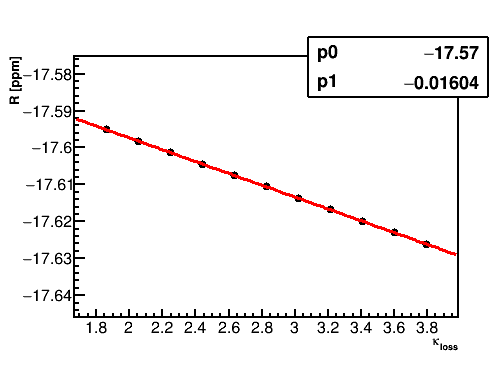
\includegraphics[width=.5\textwidth]{FullRatio_R_Vs_kappa_loss_Canv}
    \caption[Scan over fixed \K in ratio fit]{The sensitivity of \R to the fixed \K parameter. Error bars have been removed from the plot in order to show the trend more clearly. Units are in ppm per unit \K. Data are from the 9d dataset.}
    \label{fig:kappaLossScan}
\end{figure}


\begin{table}[h]
\centering
\renewcommand{\arraystretch}{1.2}
\begin{tabular*}{0.75\linewidth}{@{\extracolsep{\fill}}lGcJG}
  \hline
    \multicolumn{5}{c}{\textbf{Fixed $\kappa_{loss}$ Systematic Uncertainty}} \\
  \hline\hline
    Dataset & \multicolumn{1}{c}{$dR/d\kappa_{loss}$} &  \thead{T-Method \K} & \multicolumn{1}{c}{$\boldsymbol{\delta R}$} & \multicolumn{1}{c}{$\Delta R_{\text{(w/ - w/o)}}$} \\
  \hline
    60h & -3.06 & $8.253 \pm 0.305$ & 0.9 & -26.1 \\
    HighKick & -8.74 & $4.014 \pm 0.391$ & 3.4 & -35.1 \\
    9d & -16.04 & $2.826 \pm 0.193$ & 3.1 & -45.3 \\
    Endgame & +1.43 & $2.634 \pm 0.041$ & 0.1 & +3.8 \\
  \hline
\end{tabular*}
\caption[]{Systematic uncertainty due to the fixed $\kappa_{loss}$ parameter in the R-Method fits. All units are in ppb except for \K which is unit-less. $\sigma_{\kappa_{loss}}$ comes from the T-Method fit results and scales down with the number of statistics. The bold column gives the systematic uncertainties on \R. The far right column gives the change in $R$ with the \K parameter in the fits versus without it entirely.}
\label{tab:systematicError_kappaLoss}
\end{table}
